\begin{definition} Скалярное произведение

    $H$ --- векторное пространство,
    $\dotprod{\cdot}{\cdot}: H \times H \to \C$ со свойствами:
    \begin{enumerate}
        \item $\dotprod{x}{x} \geq 0$ и $\dotprod{x}{x} = 0 \iff x = 0$
        \item $\dotprod{x+y}{z} = \dotprod{x}{z} + \dotprod{y}{z}$
        \item $\dotprod{x}{y} = \conj{\dotprod{y}{x}}$
        \item $\dotprod{\alpha x}{y} = \alpha \dotprod{x}{y}$, $\alpha \in \C$
    \end{enumerate}
\end{definition}

\begin{observation}
    $\norm{x} := \sqrt{\dotprod{x}{x}}$ --- норма.
\end{observation}

\begin{definition}
    $H$ --- гильбертово пространство, если в нем есть скалярное произведение и $H$ --- полное.
\end{definition}

\begin{examples}
    \begin{enumerate}
        \item $L^2(E, \mu)$, $\dotprod{f}{g} := \int\limits_E f(x)\conj{g(x)} d\mu(x)$
        \item $\ell^2$ --- последовательности чисел, т.ч. $\sum \cdot^2$ конечны.

              $\dotprod{x}{y} := \sum \limits_{n=1}^\infty x_n\conj{y_n}$
    \end{enumerate}
    Полноту этих пространств уже проверяли.
\end{examples}

\begin{lemma}
    $\sum\limits_{n=1}^\infty x_n$ сходится $\Rightarrow \dotprod{\sum\limits_{n=1}^\infty x_n}{y} =
        \sum\limits_{n=1}^\infty \dotprod{x_n}{y}$
\end{lemma}
\begin{proof}
    $S_n := \sum\limits_{k=1}^n x_k$, $S := \sum\limits_{k=1}^\infty x_k$

    Сходимость $x_n \Rightarrow \norm{S_n - S} \to 0$.

    \[
        \dotprod{S}{y} \leftarrow \dotprod{S_n}{y} = \dotprod{\sum\limits_{k=1}^n x_k}{y}
        = \sum\limits_{k=1}^n \dotprod{x_k}{y} \rightarrow \sum\limits_{k=1}^\infty \dotprod{x_k}{y}
        .\]

    Левая стрелка: $\dotprod{S_n}{y} - \dotprod{S}{y} = \dotprod{S_n - S}{y} \xrightarrow{?} 0$.

    $\abs{\dotprod{S_n - S}{y}} \leq \norm{S_n - S} \norm{y} \to 0$
\end{proof}

\begin{definition}
    Векторы $x$ и $y$ ортогональны ($x \perp y$), если $\dotprod{x}{y} = 0$.
\end{definition}
\begin{definition}
    $\sum\limits_{n=1}^\infty x_n$ --- ортогональный ряд, если
    $\dotprod{x_k}{x_j} = 0\quad \forall k \neq j$.
\end{definition}

\begin{theorem}
    $\sum x_n$ --- ортогональный ряд. Тогда он сходится $\iff \sum\limits_{n=1}^\infty \norm{x_n}^2$ сходится.
    И в этом случае $\norm{\sum x_n}^2 = \sum \norm{x_n}^2$.
\end{theorem}
\begin{proof}
    $S_n := \sum\limits_{k=1}^n x_k$, $C_n := \sum\limits_{k=1}^n \norm{x_k}^2$.

    \[\norm{S_n - S_m}^2 = \dotprod{\sum\limits_{k=m+1}^n x_k}{\sum\limits_{k=m+1}^n x_k}
        = \sum\limits_{k=m+1}^n \dotprod{x_k}{x_k} = \sum\limits_{k=m+1}^n \norm{x_k}^2 = |C_n - C_m|
    \]

    Сходится ряд из $x$'ов, значит $S_n$ имеет предел, значит она фундаментальна, а тогда $C_n$ тоже фундаментальна и имеет предел (есть полнота и в $H$ и в $\R$). В обратную сторону аналогично.

    \[\norm{\sum\limits_{k=1}^\infty x_k}^2 = \dotprod{\sum\limits_{k=1}^\infty x_k}{\sum\limits_{j=1}^\infty x_j}
        = \sum\limits_k \sum\limits_j \dotprod{x_k}{x_j} = \sum\limits_k \dotprod{x_k}{x_k} = \sum\limits_k \norm{x_k}^2
    \]
\end{proof}

\begin{consequence}
    $\sum x_n$ --- сходящийся ортогональный ряд, $\vp \in S_\N$ (перестановка).
    Тогда $\sum x_{\vp(n)}$ тоже сходится и к той же самой сумме.
\end{consequence}
\begin{proof}
    Исходный ряд сходится, значит сходится ряд из квадратов норм, в таком ряду можно переставлять члены, а тогда ряд с перестановкой тоже сходится.

    \begin{align*}
        \norm{\sum x_n - \sum x_{\vp(n)}}^2 & = \dotprod{\sum (x_n - x_{\vp(n)}}{\sum (x_k - x_{\vp(k)})}                                                                                 \\
                                            & = \sum\limits_n \sum\limits_k \dotprod{x_n}{x_k} - \dotprod{x_{\vp(n)}}{x_k} - \dotprod{x_n}{x_{\vp(k)}} + \dotprod{x_{\vp(n)}}{x_{\vp(k)}} \\
                                            & = \sum\limits_n \norm{x_n}^2 - \norm{x_{\vp(n)}}^2 - \norm{x_n}^2 + \norm{x_{\vp(n)}}^2                                                     \\
                                            & = 0
    \end{align*}
    $\Rightarrow \sum x_n = \sum x_{\vp(n)}$
\end{proof}

\begin{definition}
    $x_1, x_2, \ldots$ --- ортогональная система, если $x_i \perp x_j$ при $i \neq j$ и $x_i \neq 0 \quad \forall i$.
\end{definition}
\begin{definition}
    $x_1, x_2, \ldots$ --- ортонормированная система, если $x_i \perp x_j$ при $i \neq j$ и $\norm{x_i} = 1\quad \forall i$.
    То есть $\dotprod{x_i}{x_j} = \delta_{ij}$ хаха это функция кронекера поняли да функция кронекера наконец-то пригодилась хаха
\end{definition}

\begin{observation}
    Ортогональная система линейно независима
\end{observation}
\begin{proof}
    От противного. $\alpha_1 x_1 + \ldots + \alpha_n x_n = 0$.

    Тогда $\dotprod{\alpha_1 x_1 + \ldots \alpha_n x_n}{x_k} = 0 \quad \forall k$.
    Но $\dotprod{\cdot}{x_k} = \alpha_k \norm{x_k}^2 = 0 \Rightarrow \alpha_k = 0$.
\end{proof}

\begin{examples} Ортогональные системы.
    \begin{enumerate}
        \item $e_n = (0, \ldots, 0, 1, 0, 0, \ldots)$ (на $n$-й позиции). Это ортонормированная система в $\ell^2$.
        \item $1, \cos t, \sin t, \cos 2t, \sin 2t, \ldots$ в $L^2[0, 2\pi]$ --- ортогональная система.
        \item $e^{i n t}$ при $n \in \Z$ в $L^2[0, 2\pi]$ --- ортогональная система.

              $\frac{e^{int}}{\sqrt{2\pi}}$ --- ортонормированная.
        \item $1, \cos t, \cos 2t, \cos 3t, \ldots$ в $L^2[0, \pi]$ --- ортогональная система.

              $\sin t, \sin 2t, \sin 3t, \ldots$ в $L^2[0, \pi]$ --- ортогональная система.
    \end{enumerate}
\end{examples}

\begin{theorem}
    Пусть $\set{e_n}$ --- ортогональная система в гильбертовом пространстве $H$.

    $x = \sum\limits_{n=1}^\infty c_n e_n$ --- сходящийся ряд.

    Тогда $c_k = \dfrac{\dotprod{x}{e_k}}{\norm{e_k}^2}$.
\end{theorem}
\begin{proof}
    \[
        \dotprod{x}{e_k} = \dotprod{\sum c_n e_n}{e_k} = \sum\limits_n \dotprod{c_n e_n}{e_k} = \dotprod{c_k e_k}{e_k} = c_k \norm{e_k}^2
        .\]
\end{proof}

\begin{definition}
    $x \in H$ --- гильбертово пространство.

    $c_k(x) := \dfrac{\dotprod{x}{e_k}}{\norm{e_k}^2}$ --- коэффициент Фурье вектора $x$.

    $\sum\limits_{n=1}^\infty c_n(x) e_n$ --- ряд Фурье для вектора $x$.
\end{definition}

\begin{observation}
    \begin{enumerate}
        \item Если $x = \sum\limits_{n=1}^\infty c_n e_n$, то это его ряд Фурье.
        \item $k$-ое слагаемое в ряде Фурье

              $c_k(x) e_k = \dfrac{\dotprod{x}{e_k}}{\norm{e_k}^2} e_k$ --- проекция $x$ на прямую в направлении $e_k$.

              $x = c_k(x)e_k + z$, где $z \perp e_k$.
    \end{enumerate}
\end{observation}

\begin{theorem}{Свойства частичных сумм ряда Фурье}

    Пусть $\set{e_n}$ --- ортогональная система в гильбертовом пространстве $H$, $x \in H$.

    $S_n := \sum\limits_{k=1}^n c_k(x) e_k$,
    $\L_n := \Lin(e_1, \ldots, e_n)$.

    Тогда
    \begin{enumerate}
        \item $S_n$ --- ортогональная проекция $x$ на $\L_n$, т.е. $x = S_n + z$, $z \perp \L_n$
        \item $S_n$ --- наилучшее приближение к $x$ в $\L_n$, т.е. $\norm{S_n - x} = \min\limits_{y \in \L_n} \norm{y-x}$
        \item $\norm{S_n} \leq \norm{x}$
    \end{enumerate}
\end{theorem}
\begin{proof}
    \begin{enumerate}
        \item $z := x - S_n$, надо доказать, что $z \perp e_k, k = 1,\ldots, n$.

              $\dotprod{z}{e_k} = \dotprod{x}{e_k} - \dotprod{S_n}{e_k} = \dotprod{x}{e_k} - c_k(x)\dotprod{e_k}{e_k} = 0$
        \item $x-y = S_n - y + z$

              $\norm{x - y}^2 \underset{\perp}{=} \norm{S_n - y}^2 + \norm{z}^2 \geq \norm{z}^2$
              и равенство $\iff S_n = y$.
        \item $x = S_n + z$ и $z \perp S_n \Rightarrow \norm{x}^2 = \norm{S_n}^2 + \norm{z}^2 \geq \norm{S_n}^2$
    \end{enumerate}
\end{proof}

\begin{consequence}{Неравенство Бесселя}

    $\sum\limits_{k=1}^\infty \abs{c_k(x)}^2 \norm{e_k}^2 \leq \norm{x}^2$

\end{consequence}
\begin{proof}
    \[
        \norm{x}^2 \geq \norm{S_n}^2 = \norm{\sum\limits_{k=1}^n c_k(x) e_k}^2 \underset{\perp}{=} \sum\limits_{k=1}^n \norm{c_k(x) e_k}^2 = \sum\limits_{k=1}^n \abs{c_k(x)}^2 \norm{e_k}^2
        .\]
    Верно $\forall n$, значит в пределе тоже.
\end{proof}

\begin{theorem}{Рисса-Фишера}

    $\set{e_n}$ --- ортогональная система в гильбертовом пространстве $H$.

    Тогда
    \begin{enumerate}
        \item ряд Фурье для вектора $x \in H$ сходится
        \item $x = \sum\limits_{n=1}^\infty c_n(x)e_n + z$, где $z \perp e_n \quad \forall n \in \N$
        \item $x = \sum\limits_{n=1}^\infty c_n(x)e_n \iff \norm{x}^2 = \sum\limits_{n=1}^\infty \abs{c_n(x)}^2 \norm{e_n}^2$
    \end{enumerate}
\end{theorem}
\begin{proof}
    \begin{enumerate}
        \item $\sum\limits_{n=1}^\infty \norm{c_n(x)e_n}^2 = \sum\limits_{n=1}^\infty \abs{c_n(x)}^2 \norm{e_n}^2 \leq \norm{x}^2$ (нер-во Бесселя)
        \item $z := x - \sum\limits_{n=1}^\infty c_n(x)e_n$

              $\dotprod{z}{e_n} = \dotprod{x}{e_n} - \sum\limits_{k=1}^\infty c_k(x) \dotprod{e_k}{e_n} = \dotprod{x}{e_n} - c_n(x) \dotprod{e_n}{e_n} = 0$
        \item $\Rightarrow$ --- было ($\sim$ начало параграфа).

              $\Leftarrow$: через п.2.

              $\norm{x}^2 = \sum\limits_{n=1}^\infty \abs{c_n(x)}^2 \norm{e_n}^2 + \norm{z}^2 \Rightarrow z = 0$
    \end{enumerate}
\end{proof}

\begin{observation}
    \begin{enumerate}
        \item $\norm{x}^2 = \sum\limits_n \abs{c_n(x)}^2 \norm{e_n}^2$ --- тождество Парсеваля.
        \item $\sum\limits_{n=1}^\infty c_n(x) e_n$ --- проекции $x$ на $\Cl \Lin \set{e_1, \ldots}$ (частичные суммы в $\Lin$, а предел в замыкании).
        \item Если $\sum \abs{c_n}^2 \norm{e_n}^2 < +\infty$, то найдется $x \in H: c_n = c_n(x)$
    \end{enumerate}
\end{observation}

ч

\begin{example}{Функции Радемахера}

    $r_n(t) := (-1)^{[2^nt]}$, $t \in (0, 1)$

    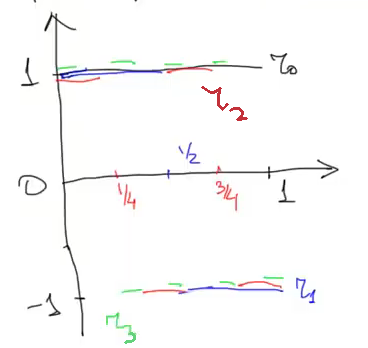
\includegraphics[width=0.5\textwidth]{complex/res/shumaher_rademaher}

    $r_n$ --- ортонормированная система в $L^2[0,1]$.
    Это \textbf{не}полная система. $r_1 r_2 \perp r_n \forall\ n$.
    Сделаем из этих функция полную систему.
\end{example}

\begin{example}{Функции Уолша}

    $A \subset \N$, $|A| < \infty$.

    $w_A(t) := \prod_{k \in A} r_k(t)$, $w_{\emptyset}(t) \equiv 1$ --- полная ортонормированная система.

    \[\dotprod{w_A}{w_B} = \int\limits_0^1 w_A w_B = \int\limits_0^1 w_{A \triangle B} = \int\limits_0^1 r_{k_1} \cdots r_{k_m} = 0
        .\]
    Считаем, что $k_i$ растут. Фиксируем $r_{k_1} \cdots r_{k_{m-1}}$, смотрим как меняется $r_{k_m}$. На половинке участков фиксированного произведения $r_{k_m} = 1$, на других половинках $-1$.

    Поймем полноту. Покажем, что $\Cl \Lin \set{w_A} = L^2[0,1]$.

    $\Lin \set{w_A\ \mid\ A \subset \set{1, \ldots, n}}$ --- пространство размерности $2^n$.
    Функции из этой линейной оболочки фиксированы на отрезках длины $2^{-n}$.
    Поэтому эта линейная оболочка содержится в $\Lin \set{\mathbbm{1}_{[\frac{k-1}{2^n}, \frac{k}{2^n})}}$, чья размерность тоже $2^n$, значит эти пространства совпадают.

    А тогда (снимаем ограничение по $n$, это типа линейная оболочка объединений по всем $n$ штук выше?) $\Lin \set{w_A} = \Lin \set{\mathbbm{1}_{[\frac{k-1}{2^n}, \frac{k}{2^n})}\ \mid\ n \in \N, 1 \leq k \leq 2^n}$ --- всевозможные ступенчатые функции с двоично-рациональными концами ступенек. А тогда замыкания этих пространств будут $L^2[0,1]$.
\end{example}

Рассмотрим $w: (a, b) \rightarrow [0, +\infty)$ ~--- измеримая, это какая-то плотность.
 $\mu A := \int_A w d\lambda$
 
 $t^k w$ суммируемы на $(a,b)$ (хотим так)
 
 Рассмотрим $L^2((a, b), \mu)$, на этом пространстве есть скалярное произведение
 $\dotprod fg := \int_a^b f\overline{g} w d\lambda$
 
 Если $\dotprod fg = 0$, то $f$ и $g$ ортогональны на $(a, b)$ с весом $w$
 
 Проделаем такое действие: возьмем последовательность мономов $1, t, t^2, \ldots$ и запустим
  на ней ортогонализацию Грама-Шмидта, получим многочлены, ортогональные на $(a, b)$ с весом $w$
  
  \begin{examples} (Ортогональных многочленов)
  	\begin{enumerate}
		\item $L^2[-1, 1]$ многочлены Лежандра, определяются как $P_k(t) := \frac{1}{2^k k!}((t^2 - 1)^k)^{(k)}$ ~--- ортогональная система.
		
		\begin{proof}
		$(k < n)$ $\int_a^b P_k P_n d\lambda = c  \int_{-1}^1 ((t^2 - 1)^k)^{(k)}((t^2 - 1)^n)^{(n)} d\lambda
		=$
		
		$  c((t^2 - 1)^k)^{(k)}((t^2 - 1)^n)^{(n - 1)} \Big|_{t = -1}^{t = 1} -
		 c \int_{-1}^1 ((t^2 - 1)^k)^{(k + 1)}((t^2 - 1)^n)^{(n - 1)} d\lambda =$
		 
		 $ -
		 c \int_{-1}^1 ((t^2 - 1)^k)^{(k + 1)}((t^2 - 1)^n)^{(n - 1)} d\lambda =$
		 
		 $c \int_{-1}^1 ((t^2 - 1)^k)^{(k + 2)}((t^2 - 1)^n)^{(n - 2)} d\lambda = \ldots =
		 \pm c \int_{-1}^1 ((t^2 - 1)^k)^{(2k + 1)}((t^2 - 1)^n)^{(n - k - 1)} d\lambda= 0$
		 \end{proof}
		 
		 \item $\frac{1}{\sqrt{1 - t^2}}$ на $[-1, 1]$ многочлены Чебышева 1го рода 
		 $T_k(t) = \cos(k\arccos t)$
		 
		 \begin{proof}
		$\int_{-1}^1 T_k T_n \frac{dt}{\sqrt{1 - t^2}} =  / x = \arccos t, dx = \frac{dt}{\sqrt{1 - t^2}}/ =
		\int_{-\pi}^\pi \cos(kx)\cos(nx)dx = 0$
		
		 \end{proof}
		 
		  \item $\sqrt{1 - t^2}$ на $[-1, 1]$ многочлены Чебышева 2го рода 
		 $\mathcal{U}_k(t) = \frac{\sin((k+1)\arccos t)}{\sqrt{1-t^2}}$
		 
		 \item Многочлены Эрмита 
		 $H_n(t) = e^{t^2}(e^{-t^2})^{(n)}$ ортогональны на $\mathbb{R}$ с весом $e^{-t^2}$
		 
		 \item Многочлены Лаггера $L_n(t) = \frac{1}{n!}e^t(t^n e^{-t})^{(n)}$ ортогональны на
		 $[0, +\infty)$ с весом $e^{-t}$
	\end{enumerate}
  \end{examples}
  
  \begin{definition}
   $(X, \rho)$ ~--- метрическое пространство $A\subset X$, $x\in X$
   
   Величина $E_A(x) := \rho(x, A) = \inf_{y \in A} \rho(x, y)$ называется наилучшим приближением
   к $x$ в множестве $A$.
  \end{definition}
  
  \begin{definition}
   Если есть $y^*\in A$, такое что $\rho(x, y^*) = \rho(x, A)$, то $y*$ ~--- элемент наилучшего
   приближения к $x$ в множестве $A$
  \end{definition}
  
  \begin{theorem}(о существовании наилучшего приближения в гильбертовом пространстве)
  
  $A$ непустое, замкнутое и выпуклое подмножество $H$ ~--- гильбертово пространство, $x\in H$.
  Тогда существует единственный элемент наил. прибл. к $x$ в мн-ве $A$.
  \end{theorem}
  
  \begin{lemma}
  $\|x + y\|^2 + \|x-y\|^2  = 2 \|x\|^2 + 2\|y\|^2$
  \end{lemma}
  
  \begin{proof}
  $d := \rho(x, A)$. Пусть $y, z \in A$ $\Rightarrow$ $\frac{y + z}{2}\in A$
  
  $\|2x -y - z\|^2 + \|y - z\|^2 = 2\|x-y\|^2 + 2\|x-z\|^2$ ($\|2x - y - z\|^2 = 4\|x - \frac{y + z}{2}\|^2 \ge 4d^2$)
  
  $\Rightarrow $ $\|y - z\|^2\le 2(\|x - y\|^2 + \| x- z\|^2 - 2d^2)$
  
  Единственность. Пусть $\|x - z\| = \|x - y\| = d \Rightarrow \|y - z\|\le 0 \Rightarrow y = z$
  
  Существование. Возьмем $y_n \in A$, т.ч. $\|x - y_n\|\rightarrow d$
  
  $\|y_n - y_m\|^2 \le 2(\underset{\text{мала при бол. $n$}}{\|x - y_n\|^2  - d^2}+
   \underset{\text{мала при бол. $m$}}{\| x- y_m\|^2 - d^2})$ $\Rightarrow$ $y_n$ ~--- 
   фундаментальна $\Rightarrow y_n\rightarrow y^* \in A$
   
   $\|x - y_n\|\rightarrow \|x - y^*\| \Rightarrow \|x - y^*\| = d$
   \end{proof}
   
   \begin{theorem}(о проекции)
   
   $L$ ~--- замкнутое подпространство в гильбертовом пространстве $H$. Тогда $x$
   единственным образом представляется в виде $x = y+z$, где $y \in L$, $z \perp L$.
   При этом $y$ ~--- наилучшее приближение к $x$ в $L$.
   \end{theorem}
   
   \begin{proof}
   $y$ ~--- наилучшее приближение к $x$ в $L$, $z := x - y$.
   
   Надо доказать, что $z\perp L$. Возьмем $l\in L$ $\Rightarrow y + \lambda l \in L$
   
   $\|z - \lambda l \| = \|x - (y + \lambda l)\|^2\ge \|x - y\|^2  = \|z\|^2$, и при этом
   
   $\|z - \lambda l \| = \dotprod{z - \lambda l}{z - \lambda l} = \|z\|^2 + |\lambda|^2\| l \|^2 - \lambda\dotprod lz
   - \overline{\lambda}\dotprod zl$
   
   $|\lambda|^2\| l \|^2 - \lambda \dotprod lz - \overline{\lambda} \dotprod zl
   \ge 0$ $\forall \lambda$
   
   Подставим $\lambda = \frac{\dotprod zl}{\| l \|^2}$ и получим 
   
   $\frac{|\dotprod zl|^2}{\| l \|} - \frac{|\dotprod zl|^2}{\| l \|}
   - \frac{\overline{\dotprod zl}\dotprod zl}{\| l \|} \ge 0
   \Rightarrow \frac{|\dotprod zl|^2}{\| l \|} \le 0 \Rightarrow z\perp l$
   
   Осталось проверить единственность: Пусть $x = y + z = y' + z'$, тогда
   $L \ni y' - y = z' - z$ и при этом $z' - z\perp L$ $\Rightarrow
   \dotprod{z' - z}{z' - z} = 0 \Rightarrow z = z'$
   
   \end{proof}
   
   \begin{definition}
   Ортогональная проекция $L$ ~--- замкнутое подпространство гильбертого $H$, $x = y + z$,
   где $y \in L$ и $z \perp L$. Проекция $x$ на $L$ ~--- это $y$
   \end{definition}
   
   \begin{definition}
   Оператор ортогонального проецирования $P_L : H \rightarrow L$, $P_L x $ ~--- проекция $x$
   на $H$.
   
   Ортогональное дополнение $L$ ~--- множество векторов, ортогональных $L$. Это замкнутое
   подпространство $H$ ($L^\perp$)
   \end{definition}
   
   \begin{properties}
   \begin{enumerate}
   \item $P_L$ линеен
   
   \item $\|P_L\| = 1$, если $L \neq \{0\}$
   
   \begin{proof}
   $x = y + z$, $\|x\|^2 = \|y\|^2 + \|z\|^2 \ge \|y\|^2 \Rightarrow \|x\| \ge \|P_Lx\| \Rightarrow \|P_L\| = 1$.
   
   Если $x \in L (x\neq 0)$, то $P_Lx = x$ $\Rightarrow \|P_L\|\ge 1$
   \end{proof}
   
   \item $P_{L^\perp} = I - P_L$ ($I$ ~--- тождественный оператор)
   
   \item $(L^{\perp})^\perp = L$
   
   \begin{proof}
   $P_{(L^{\perp})^\perp} = I - P_{L^\perp} = I - (I - P_L) = P_L$
   
   $(L^{\perp})^\perp = P_{(L^{\perp})^\perp}H = P_L H = L$
   \end{proof}
   \end{enumerate}
   \end{properties}
   
   \begin{definition} $(X, \rho)$ ~--- метрическое пространство. $X$ называется сепарабельным,
   если в $X$ есть счетное всюду плотное множество.
   \end{definition}
   
   \begin{examples} $\mathbb{R}^n, \mathbb{Q}^n, L^p(\mathbb{R}^n, \lambda_n) (p < +\infty)$
   \end{examples}
   
   \begin{theorem} В любом сепарабельном гильбертовом пространстве существует счетный
   ортонормированный базис.
   
   \end{theorem}
   
   \begin{proof}
   $\{x_n\}$ ~--- счетное всюду плотное множество. Пусть $\{y_n\}$ ~--- наибольшее по 
   включению его линейно независимое подмножество. Тогда $\Lin\{y_n\} = \Lin\{x_n\}$.
   
   Применим к $\{y_n\}$ ортогонализацию Грама-Шмидта, получится $\{e_n\}$ 
   ортонормированная система.  $\Lin\{e_n\} = \Lin\{y_n\} = \Lin\{x_n\}$
   
   $\Cl \Lin\{e_n\} = \Cl \Lin\{x_n\} \supset \Cl \{x_n\} = H \Rightarrow \{e_n\}$ ~--- базис.
   \end{proof}
   
   \begin{theorem} Бесконечномерное сепарабельное гильбертово пространство изоморфно 
   $\ell^2$
   
   \end{theorem}
   
   \begin{proof}
       $\{x_n\}\rightarrow \{c_k(x)\}$, $\dotprod xy_H = 
       \dotprod{\{c_k(x)\}}{\{c_k(y)\}}_{\ell^2}$
   \end{proof}
